\subsection{Punto di lavoro del PMT2}

\subsubsection{Circuito di misura}
\marginpar{aggiungere disegno?}
Analizziamo i segnali del PMT2 per trovare il miglior punto di lavoro per le nostre esigenze. Prendiamo l'uscita positiva preamplificata dalla base del PMT stesso e la colleghiamo ad un formatore che restituisce un segnale di forma simile ad una  Gaussiana il cui picco è proporzionale all'energia immagazzinata. Questa è poi inviata ad un ADC a 13 bit che legge qualsiasi segnale superi una certa soglia interna.

Bisogna specificare che l'ADC in questione ha due modi di salvare le acquisizioni ed essi possono essere abilitati o disabilitati mediante un file di configurazione. Si può scegliere di salvare tutti i dati acquisiti in ordine di tempo in formato esadecimale%
\footnote{Chiameremo questo file \emph{log} come la sua estensione.}
oppure avere un file di testo con 8192 righe in cui il numero scritto in ogni riga è l'occorrenza del relativo valore in \emph{digit}%
\footnote{Chiameremo questo file \emph{istogramma} per non confonderlo con il precedente.}.

\subsubsection{Ricerca delle condizioni ottimali}

Facciamo questo test ponendo il PMT2 a varie distanze di fronte al collimatore.
\marginpar{sto supponendo che la descrizione dell'apparato sia stata fatta in una sezione precedente}
Ci accorgiamo, guardando l'istogramma, che è molto sensibile alle variazioni della tensione  di alimentazione. Per esempio, passando da \SI{600}V a \SI{575}V, l'energia acquisita si dimezza. Portiamo il fotopicco del cobalto ad \SI{1.33}{MeV} vicino al nostro fondoscala variando il guadagno del formatore in modo da poter analizzare il più ampio intervallo possibile di energia al di sotto di esso. Abbiamo operato questa scelta perché è il fotopicco più energetico rispetto alle altre sorgenti radioattive che useremo in seguito per calibrare il PMT2. Avendo esso una forma Gaussiana, abbiamo fatto in modo che la sua coda non finisse troppo vicina al fondoscala dell'ADC in modo da poterla fittare senza problemi. \marginpar{ci contesteranno il verbo ``fittare''?}
Dopo varie prove decidiamo di alimentare il PMT2 a \SI{650}V.

%%%%%%%%%%%%%%%%%%%%%%%%%%%%%%%%%%%%%%%%%%%%%%%%%%%%%%%%%%%

\subsection{Scintillatore plastico}

Poniamo uno scintillatore plastico (PMT1) davanti alla sorgente in modo che i raggi $\gamma$ dei fotopicchi possano interagire con gli elettroni della targhetta e subire scattering Compton. Guardiamo allora i segnali del PMT2 a vari angoli.


\subsubsection{Trigger}

Prima di esporre i risultati ottenuti, illustriamo il funzionamento del circuito adoperato.\\
Vogliamo acquisire i segnali ogni volta che l'uscita negativa di breve durata (qualche \si{ns}) del PMT2 supera una certa soglia. L'ampiezza tipica di questo segnale vale \SI{20}{mV}, perciò deve essere amplificata per poter essere letta dal discriminatore a nostra disposizione che ha una soglia minima di \SI{35}{mV}. Colleghiamo allora questa uscita ad una amplificatore 10x 
\marginpar{spero che gradiscano la notazione ``10x'' \\  ci vuole anche il disegno}
e mandiamo poi il segnale al solito discriminatore con soglia al minimo.

Per registrare il segnale dobbiamo provvedere alla costruzione di un trigger per l'ADC che, come specificato dalla documentazione, deve partire almeno \SI{200}{ns} prima del picco e deve terminare almeno \SI{200}{ns} dopo. Usando l'oscilloscopio, ritardiamo il segnale del discriminatore e lo allunghiamo attraverso l'uso di un modulo \texttt{gate \& delay} non retriggerabile. Scegliamo di farlo durare \SI{550}{ns} prima e dopo il picco del formatore.

Colleghiamo il cavo coassiale che trasmette l'uscita del formatore all'ingresso ``gate'' dell'ADC facendo un parallelo con un tappino da \SI{50}{\Omega} perché questo ingresso ha una impedenza alta e il nostro accorgimento evita la deformazione del segnale.
Modifichiamo il file di configurazione in modo che l'ADC acquisisca soltanto quando il trigger è attivo. Notiamo che la soglia appena utilizzata elimina tutti i segnali inferiori ai 1000 digit. 

\subsubsection{Risultati} % titolo provvisorio

Abbiamo analizzato gli spettri a \SI{0}{\degree}, \SI{15}{\degree}, \SI{30}{\degree}, \SI{45}{\degree}, \SI{75}{\degree} e \SI{90}{\degree}. Riportiamo in \autoref{4ang} i più significativi.
Nel grafico a \SI{0}{\degree} possiamo notare i fotopicchi del cobalto accompagnati dalla spalla Compton  dell'elettrone che è generata da un'altra diffusione Compton all'interno del NaI dopo che questo è stato ionizzato dai fotoni dei fotopicchi.
\marginpar{Questa cosa o non è corretta o comunque non è chiara.
I fotoni o fanno fotoelettrico o fanno Compton,
qui sembra che facciano entrambi in fila.}
Nei grafici successivi si nota un vistoso picco a basse energie dovuto allo scattering di raggi $\gamma$ con le pareti della stanza che poi finiscono nel nostro rivelatore.
\marginpar{spiegare meglio questa situazione}
Gli ultimi due grafici evidenziano un calo della statistica all'aumentare dell'angolo come atteso dalla formula \autoref{diff} della sezione d'urto differenziale. Il fondo cambia: non mostra più la spalla Compton e diminuisce circa linearmente prima di raggiungere i fotopicchi.
\marginpar{ho messo un autoref ad una formula che sarà in qualche punto della teoria}

\begin{figure}[h]
\centering

\subfloat
{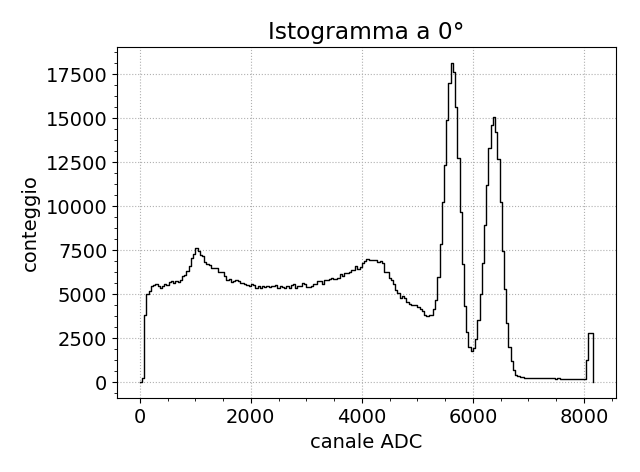
\includegraphics[width= 16 em]{0g}} \qquad
\subfloat
{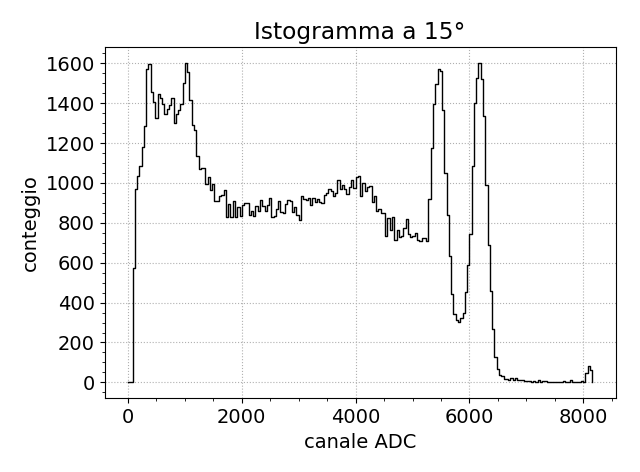
\includegraphics[width= 16 em]{15g}} \\

\subfloat
{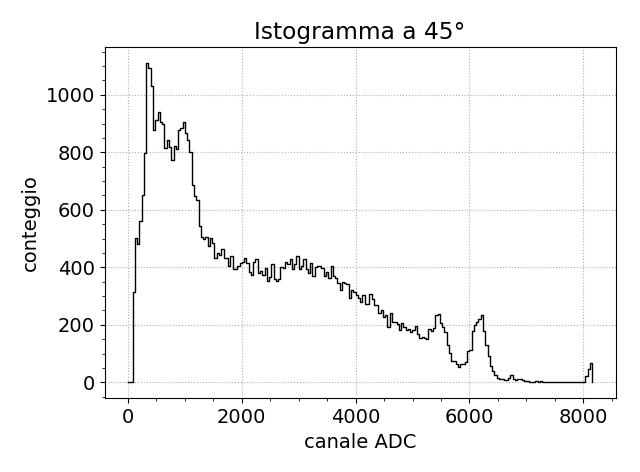
\includegraphics[width= 16 em]{45g}} \qquad
\subfloat
{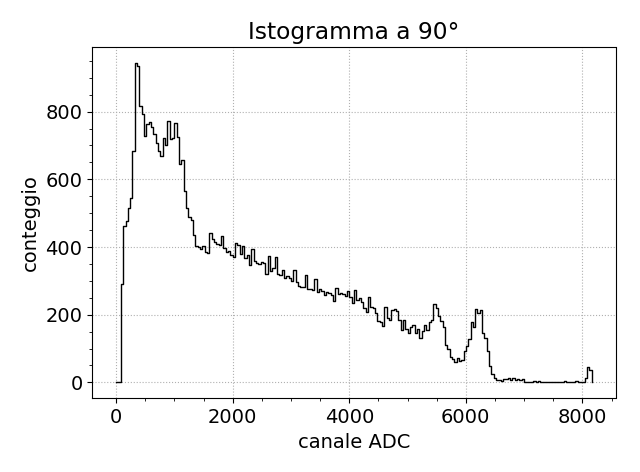
\includegraphics[width= 16 em]{90g}}

\caption{Spettri raccolti dal PMT2 a diversi angoli rispetto allo scintillatore plastico.}
\label{4ang}
\end{figure}

Abbiamo poi confrontato lo spettro a \SI{45}{\degree} con o senza scintillatore plastico, ma non abbiamo notato nessuna differenza. Abbiamo anche verificato che, come atteso, il rate di eventi diminuisce all'aumentare della distanza.
\marginpar{forse alcune di queste considerazioni sono stupide, ma è più facile togliere che aggiungere}

L'ultima acquisizione di questa serie è diversa rispetto alle altre: lo scintillatore cristallino è stato schermato lateralmente e superiormente per ridurre il backscattering. L'istogramma di \autoref{casetta} mostra come questo fenomeno sia evidentemente diventato più raro.

\begin{figure}
\centering
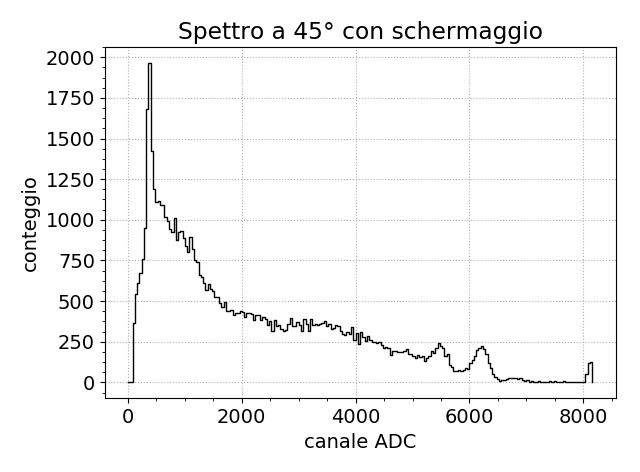
\includegraphics[width=25 em]{45gs}
\caption{Spettro energetico del PMT2 con schermaggio superiore e laterale.}
\label{casetta}
\end{figure}
